\chapter{Результаты тестирования и их анализв}
\label{chapter3}

\section{Тестовая система}
Для первоначального тестирования разработанного алгоритма использовался компьютер со следующей конфигурацией: intel core 2 duo e6550, 6GB RAM. Все вычисления производились на CPU, распараллеливание алгоритма не проводилось.

В ходе выполнения данной работы использовалось два алгоритма, реализованных в библиотеке компьютерного зрения OPenCV~\cite{opencv}: SGBM, BM. SGBM является вариацией алгоритма SGM с уменьшенным количеством оптимизируемых направлений и замененной функцией попиксельной стоимости. Алгоритм BM является представителем семейства локальных алгоритмов, скорость его выполнения значительно выше. Оба алгоритма используют дополнительные пост-процессинг шаги, в то время как в моей реализации они опущены.

Все алгоритмы реализованы на языке программирования C++~\cite{c++} с использованием библиотеки OpenCV~\cite{opencv}.

\section{Способ тестирования}
Тестирование проводилось следующим образом: для тестовой пары изображений размером [$ 384 \times 288 $] запускается алгоритм 10 раз и  подсчитывается время выполнения. Средний результат помещается в таблицу. Также в таблицу помещается качество карты диспаратности на основе онлайн бенчмарка \cite{middlebury}. Чтобы проверить верность асимптотической сложности модифицированного алгоритма, в качестве диспаратности в алгоритм передавались значения: 100, 150, 250, 300, 350.

Все реализованные мной модификации метода SGM запускались с одинаковыми параметрами. Попиксельная стоимость рассчитывалась на основе census фильтра размера [$ 5 \times 5 $]. Суммарная стоимость оптимизировалась по восьми направлениям. Остальные методы, используемые в работе, были оптимизированы для наилучшего качества.

\section{Результаты тестирования}

 Как показало тестирование, наиболее эффективный результат подсчета попиксельных стоимостей получен при предподсчете только возможных диспаратностей для каждого пикселя. Реализация, считающая стоимости во времени выполнения, не дала результатов, в связи с более частым переходам по указателям. 
\begin{table}[h!]
   \caption{Сравнение подходов подсчёта попиксельных стоимостей.}
    \label{1}
    \begin{tabular}{ | l | l | l | p{5cm} |}
    \hline
    Тип подсчета & Диспаратность & Время работы, с \\ \hline
   
    Simple & 100 & 5.0   \\ \hline
    Simple & 150 & 7.0   \\ \hline
    Simple & 250 & 8.5   \\ \hline
    Simple & 300 & 9.1  \\ \hline
    Simple & 350 & 9.7   \\ \hline
    Range & 100 & 4.7   \\ \hline
    Range & 150 & 4.8  \\ \hline
    Range & 250 & 4.7   \\ \hline
    Range & 300 & 4.7  \\ \hline
    Range & 350 & 4.7   \\ \hline
    Runtime & 100 & 6.5   \\ \hline
    Runtime & 150 & 6.6  \\ \hline
    Runtime & 250 & 6.6   \\ \hline
    Runtime & 300 & 6.7  \\ \hline
    Runtime & 350 & 6.6   \\ 
    \hline
    \end{tabular}
\end{table}

\begin{figure}[h!]
\center{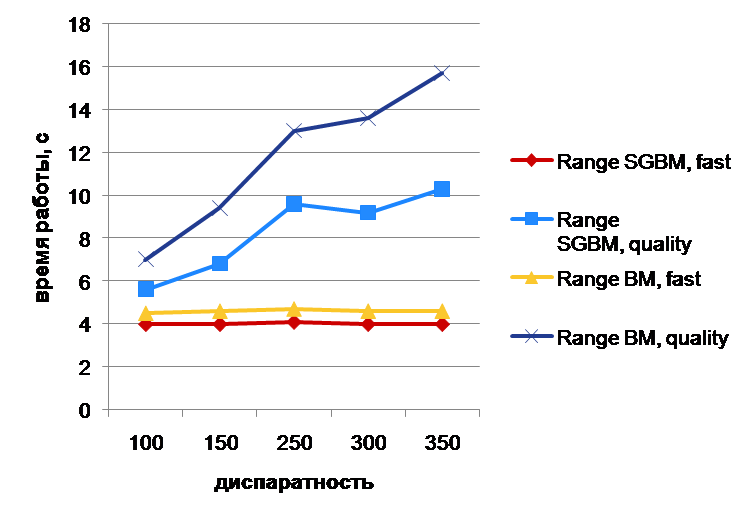
\includegraphics[scale=1]{7.png}}
\caption{Сравнение подходов подсчёта попиксельных стоимостей.}
\label{3}
\end{figure}

В табл.~\ref{1} указано время работы алгоритма на одном и том же изображении при различных типах подсчёта стоимостей, где $Simple$ - полный подсчёт всех диспаратностей перед основной частью алгоритма, $range$ - подсчёт только допустимых диспаратностей на основе приближенной карты глубины, "runtime" - подсчёт стоимости в случае потребности алгоритма. Замер производился с помощью модифицированного подхода на основе алгоритма BM. 

В ходе второго эксперимента были рассмотрены подходы задания интервала диспаратностей: $fast$ - интервал строится на основе соседнего пикселя, если мы не доверяем текущему и $quality$ - рассматривается весь интервал от $0$ до $max\_disparity$. Результат эксперимента~\ref{2} подтвердил, что подход $fast$ позволяет решать задачу построения карты глубины ассимптотически независимо от максимальной диспаратности. Также мы видим, что при подходе $quality$  имеет значение алгоритм, используемый в качестве приближения. Модифицированный метод, основанный BM, работает по времени пропорционально диспаратности, потому что у алгоритма BM существует множество точек, для которых не найдено сопоставление. График~\ref{3} иллюстрирует данные выводы.


\begin{table}[h!]
   \caption{Зависимость времени выполнения алгоритма от способа задания интервала диспаратностей.}
    \label{2}
    \begin{tabular}{ | l | l | l | p{5cm} |}
    \hline
    Алгоритм & Тип задания интервала &  Диспаратность & Время работы, с \\ \hline
   
SGBM	& FAST	& 100	& 4.0	\\ \hline
SGBM	& FAST	& 150	& 4.0	\\ \hline
SGBM	& FAST	& 250	& 4.1	\\ \hline
SGBM	& FAST	& 300	& 4.0	\\ \hline
SGBM	& FAST	& 350	& 4.0	\\ \hline
SGBM	& QUALITY	& 100	& 5.6	\\ \hline
SGBM	& QUALITY	& 150	& 6.8	\\ \hline
SGBM	& QUALITY	& 250	& 9.6	\\ \hline
SGBM	& QUALITY	& 300	& 9.2	\\ \hline
SGBM	& QUALITY	& 350	& 10.3\\ \hline	
BM		& FAST	& 100	& 4.5	\\ \hline
BM		& FAST	& 150	& 4.6	\\ \hline
BM		& FAST	& 250	& 4.7	\\ \hline
BM		& FAST	& 300	& 4.6	\\ \hline
BM		& FAST	& 350	& 4.6	\\ \hline
BM		& QUALITY	& 100	& 7.0	\\ \hline
BM		& QUALITY	& 150	& 9.4	\\ \hline
BM		& QUALITY	& 250	& 13.0\\ \hline
BM		& QUALITY	& 300	& 13.6\\ \hline
BM		& QUALITY	& 350	& 15.7\\ 
    \hline
    \end{tabular}
\end{table}

В табл.~\ref{4} представлено общее сравнение алгоритмов, а также их результаты в системе тестирования алгоритмов стереозрения~\cite{middlebury}. Из таблицы следует, что при использовании модифицированного подхода мы получаем результаты по качеству почти равные с лидером - SGM. В тоже время модифицированный алгоритм на основе BM работает в 4 раза быстрее при потери в качестве 28\%, используя $fast$, и в два раза быстрее при потере в качестве 2.8\%. Таким образом нам выгодно заменить стандартный алгоритм Semi-Global Matching на модифицированный метод на основе BM. 
\begin{table}[h!]
   \caption{Итоговое сравнение различных алгоритмов.}
    \label{4}
    \begin{tabular}{ | l | l | l | p{5cm} |}
    \hline
    Алгоритм & Время работы, с & Процент ошибок \\ \hline
     SGM & 17.4 & 10.9  \\ \hline
    SGBM & 3.8 & 11.9  \\ \hline
    BM & 0.4 &  26.2 \\ \hline
    Range by SGBM, FAST& 4.0 & 11   \\ \hline
    Range by SGBM, QUALITY & 6.7 & 11  \\ \hline
    Range by BM, FAST & 4.0 & 14.4  \\ \hline
    Range by BM, QUALITY & 8.8 & 11.2  \\ 
    \hline
    \end{tabular}
\end{table}

На рис.~\ref{pic:6},~\ref{pic:7},~\ref{pic:8} приведены примеры построенных карт с помощью различных алгоритмов. Заметим, что реализации SGM и модифицированного алгоритма не использует эвристики. А также, если мы найдем алгоритм, выдающий карту глубин с большим количеством "доверенных" пикселей, время выполнения подхода $quality$ упадет без потери качества.

\begin{figure}[h!]
\center{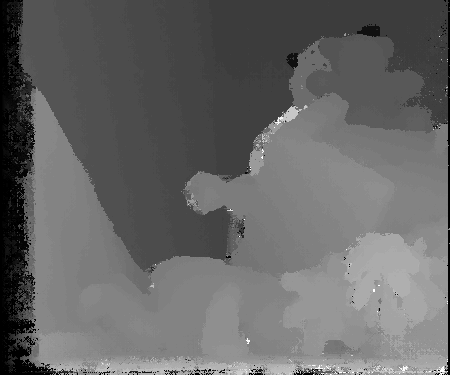
\includegraphics[scale=0.7]{teddy_RANGEbyBM.png}}
\caption{Карта глубины с основе пары изображений "teddy" с помощью модифицированного алгоритма на основе BM.}
\label{pic:6}
\end{figure}

\begin{figure}[h!]
\center{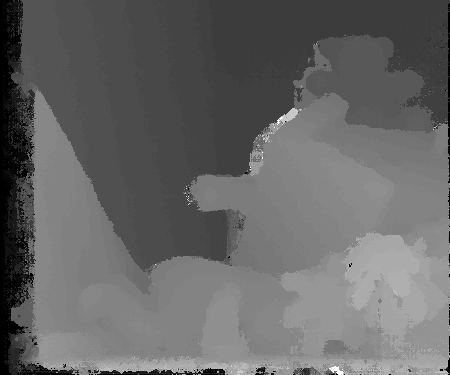
\includegraphics[scale=0.7]{teddy_RANGEbySGBM.png}}
\caption{Карта глубины с основе пары изображений "teddy" с помощью модифицированного алгоритма на основе SGBM.}
\label{pic:7}
\end{figure}

\begin{figure}[h!]
\center{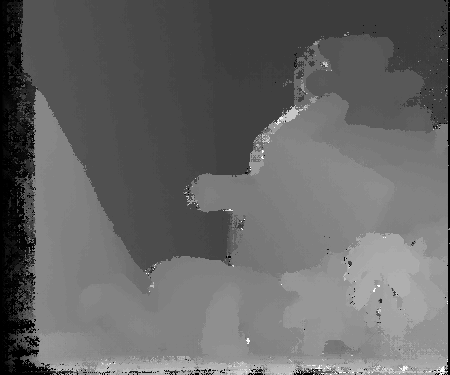
\includegraphics[scale=0.7]{teddy_SGM.png}}
\caption{Карта глубины с основе пары изображений "teddy" с помощью SGM.}
\label{pic:8}
\end{figure}

\clearpage